%!TEX root = ../../super_main.tex

\section{Vision}
\label{sec:vision}

% Vi har ikke nogen udefrakommende kunne, vi vil håndtere dette med et essence vision
This project aims to be innovative and does not have an external customer whom can define and verify requirements. 
\\\\
A methodology that aims to support high value software solutions is Essense \todo{Ref til Essence bog}. Essence mentions having a vision as a great way to start a project. Essence mentions that having different representations of a vision can help elicit objects, events, and qualities to persue. Four different representation types are suggested, namely: Icon, Prototype, Metaphor, Proposition. We have chosen to attempt to represent the existing condition, i.e. the problem area as we understood it at the time, as Icons, Metaphors, and Propositions. We found the prototype representation to costly in terms of development time. 

\subsection{Vision Scenarios}
\label{sub:vision_scenarios}

There should be four representations for each type, one for each direction of two, for the project, fundamental questions. The Essence book has an example project called Psyche where several different opposing questions were found. The two most central questions were picked and used to generate the four representation for each type. We have taken a similar approach and have come up with a list of opposing questions. 

\begin{itemize}[itemsep=0.1em]
	\item Disruptive/Non-disruptive - Should the system be based on passively collected sensor data or interactively prompt with questionnaires? % 1
	\item On demand/Continuous - Should the system be activated by users or run continuously in the background? % 2
	\item Easy-of-use/Customizable - Should we require that customers must customize campaigns or should it be ``one data collection configuration fits all''? % 3
	\item Assigned/Opt-in - Should campaigns be assigned automatically to users using a user profile or should users actively choose campaigns? % 4
	\item Personal/Anonymous - Should the system require personal information about users or not? % 5
\end{itemize}

We have chosen to use the Ease-of-use/Customizable and Assigned/Opt-in orientation questions as axes. 
\\\\
% 1
We found it difficult to imagine the usefulness of a system that exclusively collects sensor data for classification problems. This means that at least some data not based on sensor should be collected. The degree of disruptiveness could then perhaps be regulated by the campaign configuration. 
% 2
The system could allow users to turn the system on/off easily but we think that having the system running continuously once activated would increase the probability of completing campaigns. Actual data collection would also depend on whether there is one or more active campaigns on the user's device.
% 5
We found that some demographic information would be necessary for both the scenario where users are assigned to campaigns and where they opt-in. Customers would likely be interested in whether the collected data represents the wide population or the specific group they are targeting for their data collection project. The degree of personal information required for a given campaign could perhaps also be defined in a campaign configuration. 
\\\\
We have chosen to include Ease-of-use/Customizable because we thought it would be interesting to explore different 




% 1: rå sensor data har begrænset anvendelsesmuligheder --> spørgeskema kan hjælpe med dette.
% 		brug for en eller anden grad af labels fra brugere. Behøver ikke komme fra spørgeskemaer

% 2: Skal bruger forstyrres "unødvendigt" eller selv aktivt starte appen op fx. hver dag eller skal den køre i baggrunden
% Fordel ved selv styring er at de kan regulere strøm forbrug og vælge hvilke dag de vil deltage. Ulempe ved at de vælger er at det kan være svært at generalisere over tid. 
% Begge dele kan påvirker bruger entusiasmen/involveringen

% 3: Skal det være nemt/hurtigt at lave campaigns

\subsection{Icon Representation}


\subsection{Metaphor Representation}


\subsection{Proposition Representation}


\begin{figure}[!htbp]
    \centering
    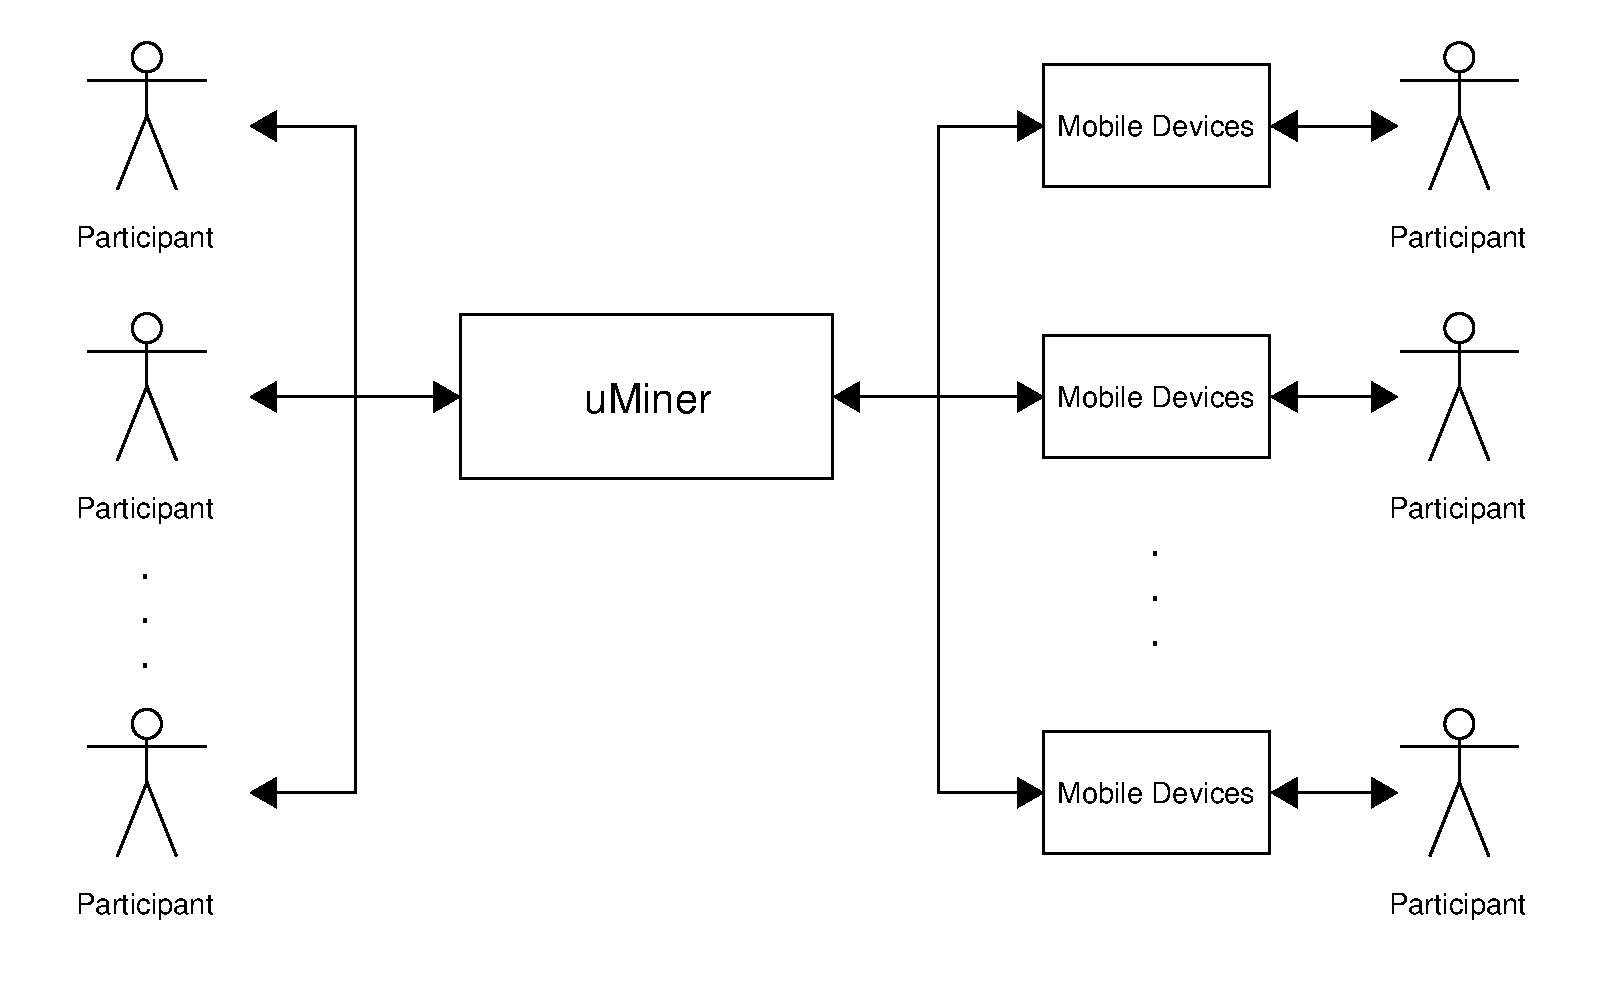
\includegraphics[width=\textwidth]{unsorted/system_vision}
    \caption{The system vision.}
    \label{fig:system_vision}
\end{figure}
\FloatBarrier
